\chapter{Implementacija i korisničko sučelje}
		
		
		\section{Korištene tehnologije i alati}
		
			Pri izradi aplikacije koristili smo bazu podataka PostgreSQL, s kojom aplikacija komunicira preko platforme za ravoj aplikacija java Spring Boot. U njoj su isprogramirane same funkcionalnosti aplikacije. Njih smo tijekom razvoja poloću slanja http zahtjeva provjeravali preko razvojnog alata Postman koji je služio kao sučelje.  Samo sučelje aplikacije je pisano u JavaScript biblioteci React. Za samo programiranje smo koristili razvojna okružja Intelij i Eclipse. Za pisanje dokumentacije smo koristili uređivački program TeXstudio, a potrebne dijagrame smo radili u UML alatu za modeliranje zvanom Astah. Za spremanje koda i dokumentacije i praćenje verzija aplikacija smo koristili internetski alat gitLab. 
		
	
		\section{Ispitivanje programskog rješenja}
			
			\subsection{Ispitivanje komponenti}
			
			Komponente su ispitane kroz njihov razvoj.
			
			\subsection{Ispitivanje sustava}
			
			\textbf{1. Ispitivanje promjene podataka profila}
			
			-ulaz : korisničko ime i lozinka korisnika 
			
			-očekivani rezultat : promjenjene vrijednosti na profilu
			
			-koraci : 
			
			\begin{packed_enum}
				
				\item ulogiramo se kao korisnik     
				\item ou kartici gdje su zapisani podaci stisnemo edit profile
				\item unesemo nove podatke i stisnemo save
				\item  aplikacija nas baci na pocetnu stranicu gdje su u kartici promjenjeni 
				
			\end{packed_enum}
			 
			 
			 
			 \textbf{2. Ispitivanje slanje suradnje između klijenta i doktora ili trenera}
			 
			 -ulaz : korisničko ime i lozinka korisnika 
			 
			 -očekivani rezultat : prikaz suranje na profilima klijenta i doktora ili trenera
			 
			 -koraci : 
			 
			 \begin{packed_enum}
			 	
			 	\item ulogiramo se kao klijent    
			 	\item u karticama Doctors ili Coaches izaberemo doktora ili trenera s kojim bi htjeli zapoceti suradnju
			 	\item pritisnemo gumb send request
			 	\item  ulogiramo se kao doktor ili trener
			 	\item prihvatimo ili odbijemo suranju pritiskom na gumb accept ili decline
			 	
			 \end{packed_enum}
		 
		 	\textbf{2. Ispitivanje prekida suranje }
		 	
		 	-ulaz : korisničko ime i lozinka korisnik 
		 	
		 	-očekivani rezultat : prekinuta suradnja
		 	
		 	-koraci : 
		 	
		 	\begin{packed_enum}
		 		
		 		\item ulogiramo se kao klijent
		 		\item u karticama my doctor ili my coach pritisnemo end collaboration
		 		
		 		
		 	\end{packed_enum}
			
			\eject 
		
		
		\section{Dijagram razmještaja}
			
			Dijagramima razmještaja prikazana je programska potpora i sklopovlje korišteno prilikom implementacije sustava. Baza podataka i web poslužitelj nalaze se na poslužiteljskom računalu. Web preglednik, pomoću kojega se pristupa aplikaciji, nalazi se na klijentskom računalu. Komunikacija između korisnika (klijent,doktor,trener,admin) odvija se preko HTTP veze. Specifikacijski dijagram razmještaja pokazuje da je sustav baziran na arhitekturi “klijent-poslužitelj”. Dijagram razmještaja instanci prikazuje sustav tijekom suradnje jednog klijenta,doktora i trenera. 
			
			\begin{figure}[h]
				\centering
				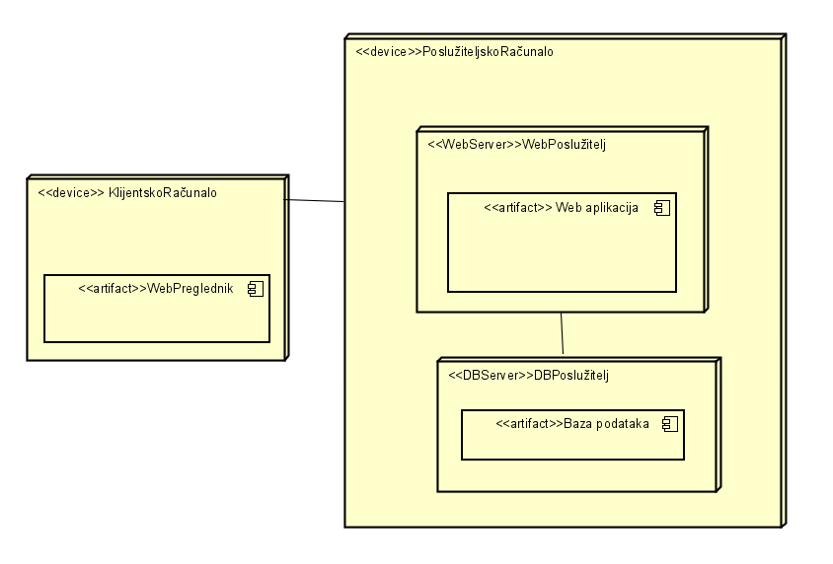
\includegraphics[scale=0.8]{dijagrami/DijagramRazmjestaja}
				\caption{Specifikacijski dijagram razmještaja}
			\end{figure}
			
			\begin{figure}
				\centering
				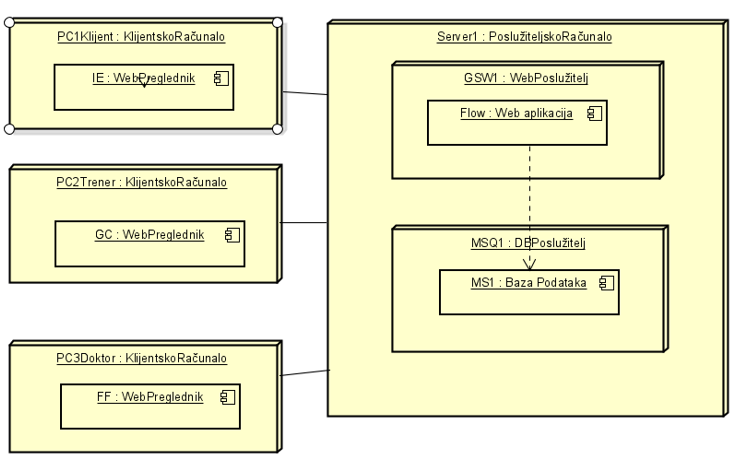
\includegraphics[scale=1]{dijagrami/DijagramRazmjestaja2}
				\caption{Dijagram razmještaja instanci}
			\end{figure}
			\eject 
		
		\section{Upute za puštanje u pogon}
		
			Ove upute su pisane za operacijski sustav Windows 10, aplikaciju je moguće pokrenuti i na drugim operacijskim sustavima, ali treba se voditi računa da se programi drukčije instaliraju na njima i da su naredbe različite.
			\\
			Potrebno je preuzeti installer datoteku s web stranice
			\\ 
			\texttt{\small https://www.postgresql.org/}
			\\
			i provesti standardnu instalaciju PostgreSQL baze podataka na računalo. Bitno je zapamtiti korisničko ime i lozinku koja se postavlja u instalaciji jer će biti potrebne za kasnije spajanje na bazu podataka. Nakon instalacije potrebno je pokrenuti \texttt{\textit{pgAdmin.exe}} koji će otvoriti sučelje za upravljanje bazama podataka.
			
		
			Zatim treba stvoriti novu bazu podataka tako da se na izborniku koji se prikaže desnim klikom na \texttt{\textit{'databases'}} odabere opcija \texttt{\textit{'Create->Database...'}}(ime je proizvoljno).
			
			\begin{figure}[h]
				\centering
				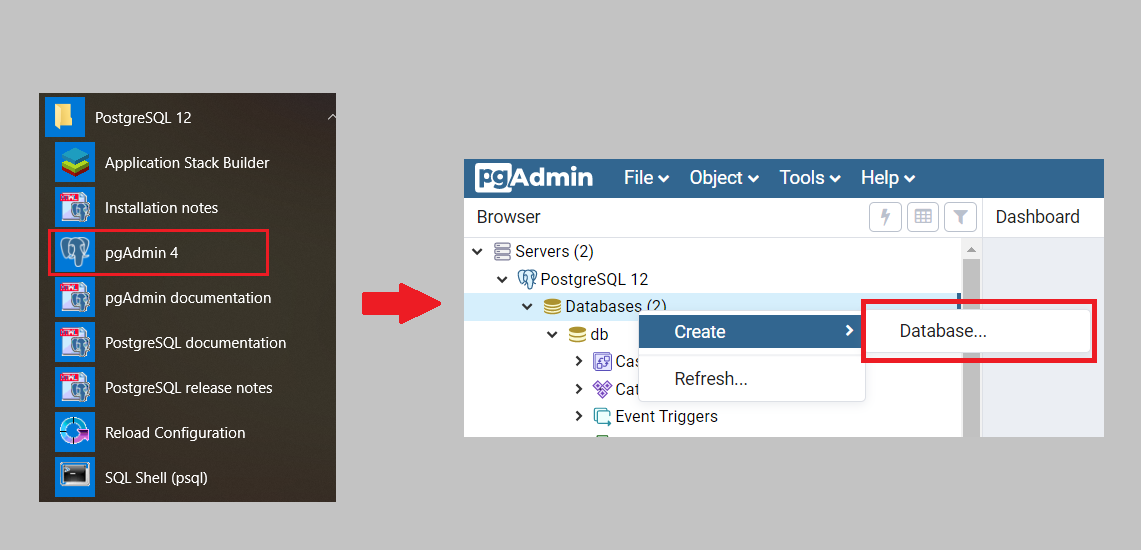
\includegraphics[scale=0.7]{slike/pustanjeupogon/a.png}
				\caption{Stvaranje baze podataka}
			\end{figure}
			
			Backend aplikacije pisan je u programskom jeziku Java, stoga računalo mora na sebi imati instaliran Java Development Kit(JDK) verzija 13. Preuzeti ga je moguće sa službene web stranice:
			\\
			\texttt{\small https://www.oracle.com/technetwork/java/javase/downloads/index.html}
			\\
			Provesti standardnu instalaciju i provjeriti je li sve ispravno instalirano tako da se otvori Command Prompt i upiše \textbf{\texttt{'java --version'}}, ako je sve uredu ispisati će se verzija instalirane jave.
			
			\begin{figure}[h]
				\centering
				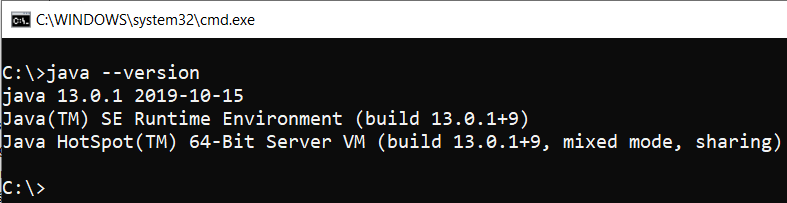
\includegraphics[scale=0.6]{slike/pustanjeupogon/javaversion.png}
				\caption{Provjera je li JDK ispravno instaliran}
			\end{figure}

			U pisanju backenda korišten je Spring framework te zato računalo mora imati instaliran Maven koji vodi računa o svim zavisnostima (dependencies) koje projekt ima. Potrebno je preuzeti zip arhivu s web stranice:
			\\
			\texttt{\small https://maven.apache.org/download.cgi}
			\\
			te ju raspakirati u željeni direktorij. Potom, podesiti environment varijable operacijskog sustava tako da otvorite \texttt{\textit{'System Properties'}} (to je moguće na par načina, ali najlakše je tako da se u polje za pretraživanje upiše: \texttt{\textit{'edit the system en...'}}) i odaberete \texttt{\textit{'Edit the system environment variables'}}.
			
			\begin{figure}[h]
				\centering
				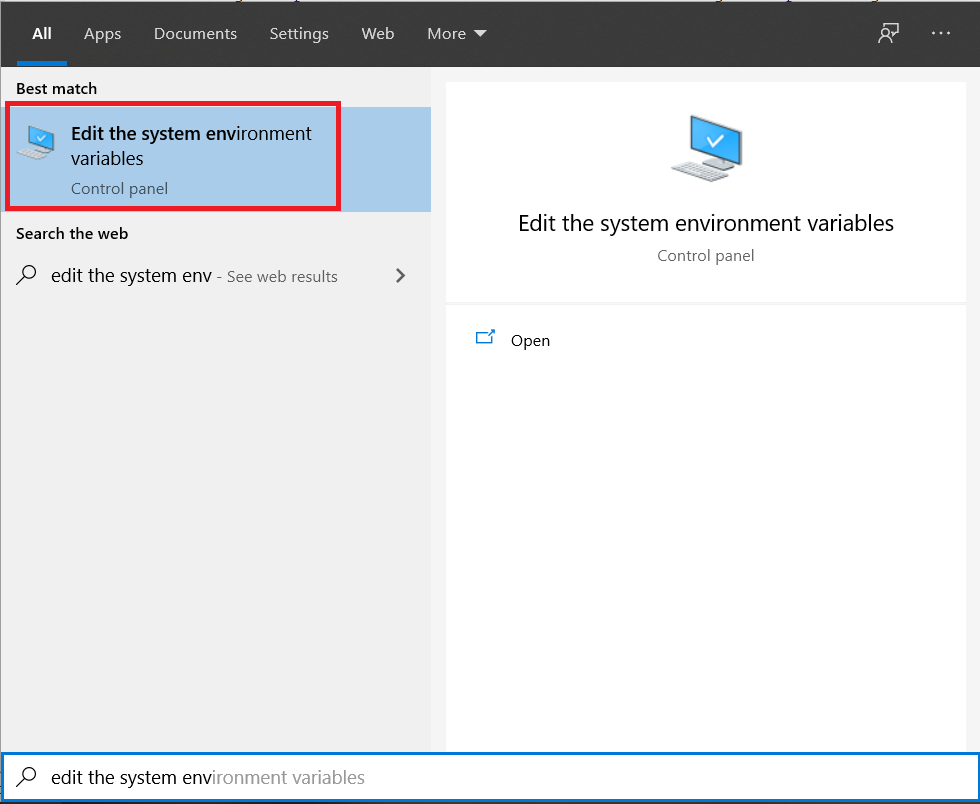
\includegraphics[scale=0.45]{slike/pustanjeupogon/search.png}
				\caption{Otvaranje System Properties}
			\end{figure}
			
			U prozoru koji se otvorio odaberite \texttt{\textit{'Environment Variables'}}, nakon toga odabrati opciju \texttt{\textit{'New'}} u dijelu sučelja \texttt{\textit{'System Variables'}}, u polje \texttt{\textit{'Variable name'}} upisati \texttt{\textit{'MAVEN\_HOME'}}, a u polje \texttt{\textit{'Variable value'}} upisati putanju direktorija koji je nastao raspakiravanjem zip arhive. Potom je potrebno odabrati opciju \texttt{\textit{'Edit'}} za varijablu \texttt{\textit{'Path'}} u polju \texttt{\textit{'System Variables'}} i kada se otvori novi prozor odabrati opciju \texttt{\textit{'New'}} te upisati \texttt{\small '\%MAVEN\_HOME\%\textbackslash bin'}. Maven bi sada trebao biti uspješno instaliran, provjeriti tako da se u Command Prompt upiše naredba \texttt{\textbf{'mvn --version'}}.
			
			\begin{figure}[h]
				\centering
				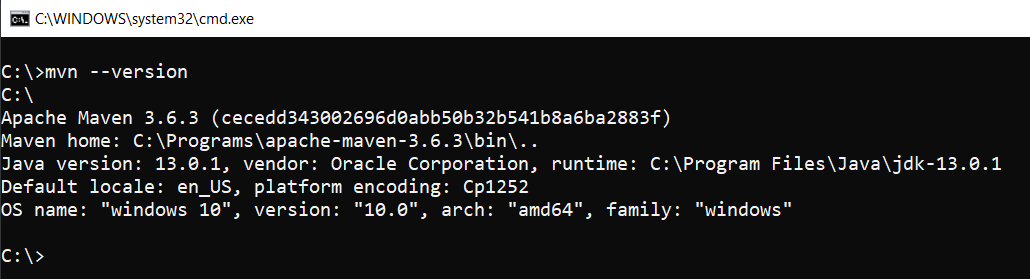
\includegraphics[scale=0.5]{slike/pustanjeupogon/mavenversion.png}
				\caption{Provjera je li Maven ispravno instaliran}
			\end{figure}
		
			Frontend aplikacije napisan je koristeći React Javascript library, stoga računalo mora imati instaliran Node.js kako bi ga mogli pokrenuti. S web stranice: 
			\\
			\texttt{\small https://nodejs.org/en/}
			\\
			preuzeti i pokrenuti installer datoteku. Provesti standardnu instalaciju. Provjeriti je li instalacija uspješna tako da se u Command Prompt upiše naredba \texttt{\textbf{'node --version'}}.
			
			\begin{figure}[h]
				\centering
				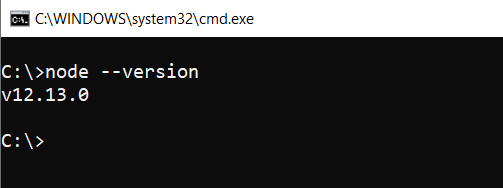
\includegraphics[scale=0.7]{slike/pustanjeupogon/nodeversion.png}
				\caption{Provjera je li Node.js ispravno instaliran}
			\end{figure}
		
			Sada kada su svi potrebni programi instalirani možemo početi s puštanjem aplikacije u pogon. Preuzeti direktorij s GitLab stranice:
			\\
			\texttt{\small https://gitlab.com/fermark/flow}
			\\
			tako da se odabere opcija \texttt{Download->zip}. Raspakirati zip arhivu te navigirati u direktorij \texttt{\small flow\textbackslash src\textbackslash main\textbackslash resources} te otvoriti datoteku \texttt{\textit{ application.properties}}. Potrebno je podesiti nekoliko parametara kako bi se moglo ispravno spojiti na bazu podataka. Za vrijednost parametra \texttt{\small <ime baze podataka>} u polju \texttt{\small spring.datasource.url} potrebno je upisati ime vaše baze podataka. U polja \texttt{\small username} i \texttt{\small password} upisati korisničko ime i lozinku koju ste odabrali kada ste instalirali PostgreSQL bazu podataka. Spremiti izmijene u datoteci.
			
			\begin{figure}[h]
				\centering
				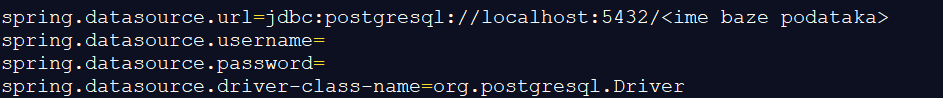
\includegraphics[scale=0.8]{slike/pustanjeupogon/app.png}
				\caption{Izmjena datoteke 'application.properties'}
			\end{figure}
			
			Otvoriti Command Prompt i navigirati u direktorij \texttt{\small \textbackslash flow} te tamo izvršiti naredbu \texttt{\textbf{'mvn install'}}. Time se stvorila izvršna datoteka tipa \texttt{'jar'} u poddirektoriju \texttt{\small target}. Sada je potrebno postaviti i frontend dio aplikacije. U Command Promptu navigirati u direktorij \texttt{\small \textbackslash flow\_front} te tamo izvršiti naredbu \texttt{\textbf{'npm install'}} koja će preuzeti biblioteku React. Potom u istome direktoriju je potrebno izvršiti naredbe \texttt{\textbf{'npm install react-router-dom --save'}} i \texttt{\textbf{'npm install axios --save'}}, a te dvije naredbe će preuzeti potrebne zavisnosti (dependecies) projekta.
			\\
			Sada još jedino preostaje pokrenuti aplikaciju. U direktoriju \texttt{\small \textbackslash flow\_front} izvršiti naredbu \texttt{\textbf{'npm start'}}, frontend dio aplikacije će se pokrenuti. Zatim je potrebno otvoriti novu instancu Command Prompta i u direktoriju \texttt{\small \textbackslash flow\textbackslash target} izvršiti naredbu \texttt{\textbf{'java -jar flow-0.0.1-SNAPSHOT.jar'}}. Ta će naredba pokrenuti backend dio aplikacije koji automatski stvara sve potrebne tablice u bazi podataka, jedino što je još potrebno napraviti je ubaciti u bazu podataka podatke za prijavu administratora. Ponovo pokrenuti sučelje za upravljanje bazom podataka \texttt{\textit{pgAdmin}} i pritisnuti desni klik na vašoj bazi podataka te odabrati opciju \texttt{\textit{Query Tool...}}.
			
			\begin{figure}[h]
				\centering
				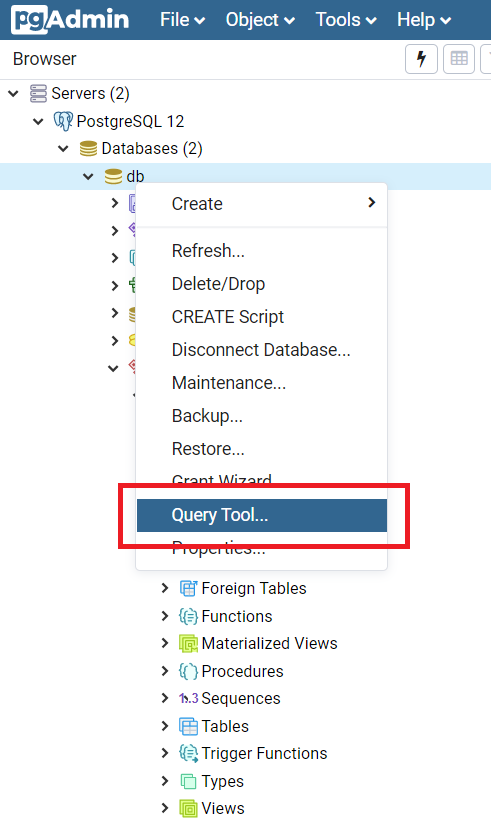
\includegraphics[scale=0.5]{slike/pustanjeupogon/query.png}
				\caption{Otvaranje Query Toola u pgAdmin sučelju}
				
			\end{figure}
			\newpage
			 U polje \texttt{\small Query Editor} upisati naredbu \texttt{\textbf{'INSERT INTO client VALUES ('1', 'ADMIN', 'ADMIN, 'ADMIN, 'ADMIN');'}} i izvršiti ju pritiskom na gumb s ikonom munje.
			
			\begin{figure}[h]
				\centering
				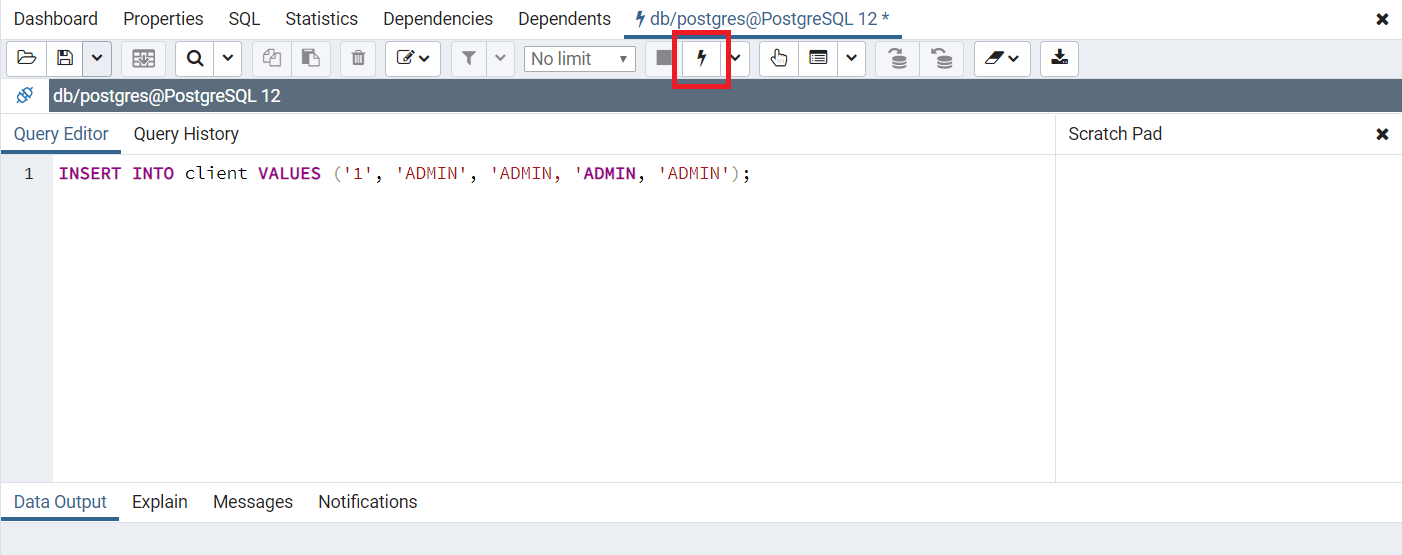
\includegraphics[scale=0.5]{slike/pustanjeupogon/insert.png}
				\caption{Izvršavanje naredbe u sučelju pgAdmin}
			\end{figure}
			
			Aplikacija je pokrenuta i moguće joj je pristupiti na URL
			\\
			\texttt{ \small http://localhost:3000/}
			
			
			\eject 